\documentclass[12pt]{beamer}
%\documentclass[20pt,handout]{beamer}
\usetheme{Darmstadt}
\usepackage{graphicx}
%\usepackage[german]{babel}
\usepackage{ngerman}
\usepackage[T1]{fontenc}
\usepackage[utf8]{inputenc}
\usepackage{tikz}
\setbeamertemplate{footline}[frame number]

\newcommand{\cc}[1]{\includegraphics[height=4mm]{img/#1.png}\hspace{1mm}}
\usepackage{ifthen}
\newcommand{\license}[2][]{\\#2\ifthenelse{\equal{#1}{}}{}{\\\scriptsize\url{#1}}}
\usepackage{textcomp}
\usepackage{hyperref}

\pgfdeclareimage[height=.6cm]{c3d2logo}{./img/c3d2.pdf}


\pgfdeclarelayer{foreground}
\pgfsetlayers{main,foreground}
\logo{\pgfputat{\pgfxy(-1,0)}{\pgfbox[center,base]{\pgfuseimage{c3d2logo}}}}


\title{Das sind doch nur Metadaten}
\author{\small Stephan Thamm\\\large Chaos Computer Club Dresden}
\date{28.09.2016}

\begin{document}
\maketitle

\section{Einleitung}
\subsection{}

\begin{frame}
  \frametitle{Chaos Computer Club}
  \begin{center}
    
\includegraphics[height=0.1\textheight]{img/c3d2_logo.png}
  \end{center}
  \begin{itemize}
    \item<1-> Chaos Computer Club Dresden (\url{https://c3d2.de})          
    \item<2-> Datenspuren: 22.10 - 23.10.2016 (\url{https://datenspuren.de})
    \item<3-> Podcasts (\url{https://c3d2.de/radio.html})
    \item<4-> Chaos macht Schule (\url{https://c3d2.de/schule.html})
  \end{itemize}
\end{frame}

\begin{frame}
  \frametitle{Metadaten}
  \only<2>{
    \begin{center}
      \fbox{
        
\includegraphics[height=0.7\textheight]{img/psb.png}
      }
    \end{center}
  }
  \only<3>{
    \begin{center}
      \large Metadaten oder Metainformationen sind Daten, die Informationen über Merkmale anderer Daten enthalten, aber nicht diese Daten selbst.
    \end{center}
  }
\end{frame}

\section{Vorratsdatenspeicherung}
\subsection{}

\begin{frame}
  \frametitle{Vorratsdatenspeicherung}
  \begin{itemize}
    \item<2-> Standortdaten der Teilnehmer aller Mobiltelefonate bei Beginn des Telefonats, zu speichern für 4 Wochen
    \item<3-> Standortdaten bei Beginn einer mobilen Internetnutzung, zu speichern für 4 Wochen
    \item<4-> Rufnummern, Zeit und Dauer aller Telefonate, zu speichern für 10 Wochen
    \item<5-> Rufnummern, Sende- und Empfangszeit aller SMS-Nachrichten, zu speichern für 10 Wochen
    \item<6-> zugewiesene IP-Adressen aller Internetnutzer sowie Zeit und Dauer der Internetnutzung, zu speichern für 10 Wochen
  \end{itemize}
\end{frame}

\begin{frame}
  \frametitle{Bewegungsdaten}
  \pause
  \begin{center}
    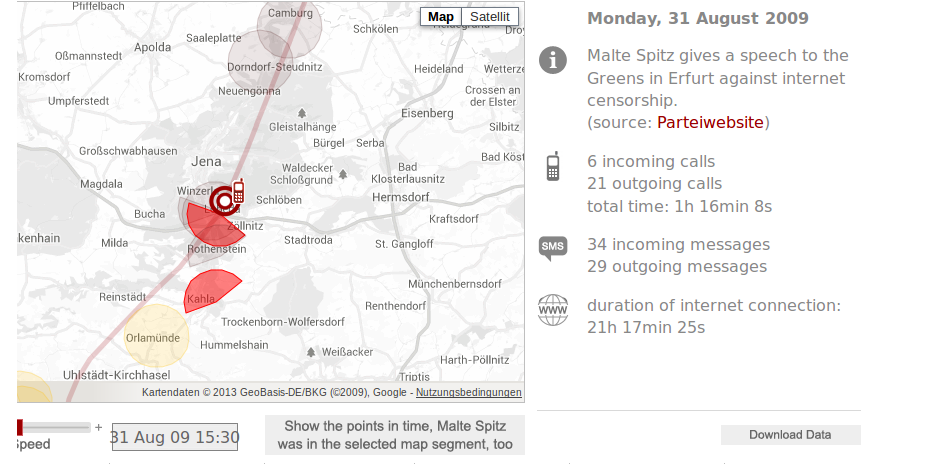
\includegraphics[height=0.7\textheight]{img/maltespitz.png}
  \end{center}
\end{frame}

\begin{frame}
  \frametitle{Verbindungsdaten}
  \begin{center}
    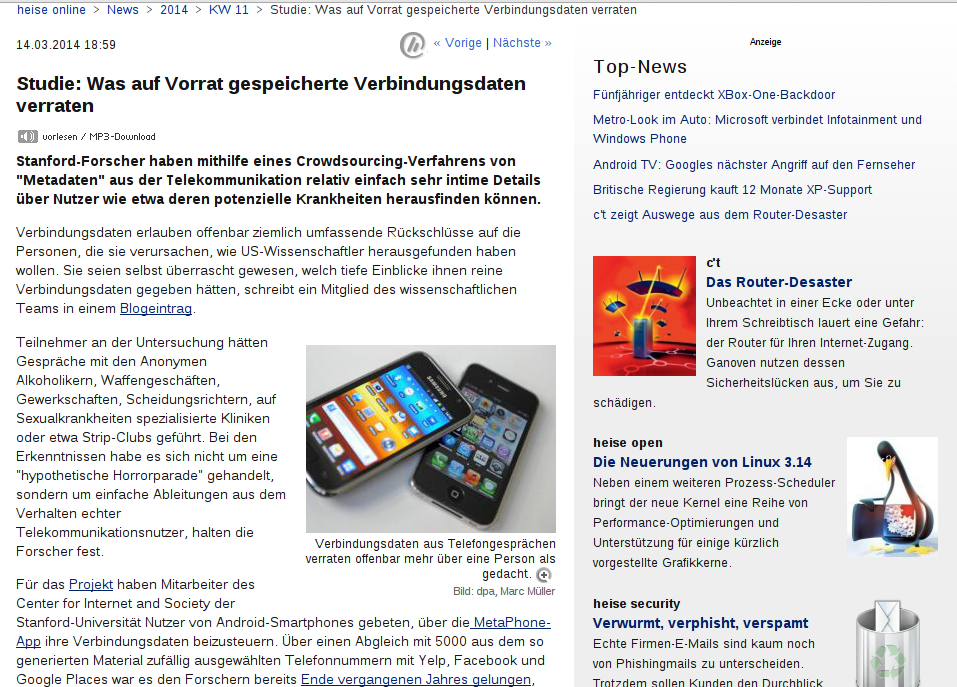
\includegraphics[height=0.7\textheight]{img/metadaten_studie.png}
  \end{center}
\end{frame}

\begin{frame}
  \frametitle{Metada Matters}
  \begin{center}
    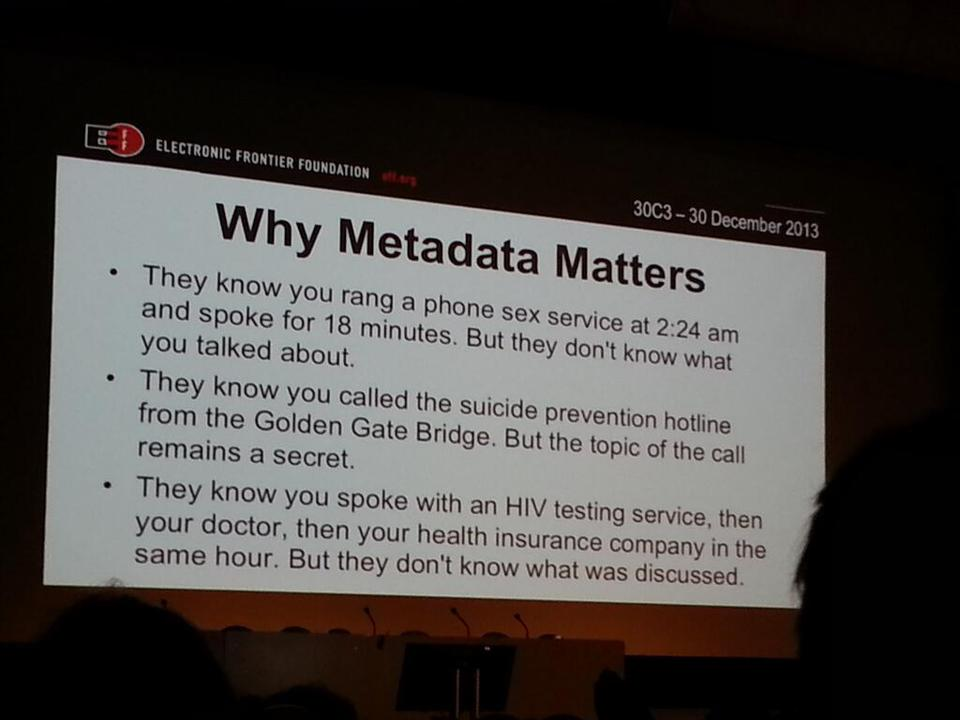
\includegraphics[height=0.7\textheight]{img/metadata-matters.jpg}
  \end{center}
\end{frame}

\section{Geheimdienste}
\subsection{}

\begin{frame}
  \frametitle{Was tun die USA mit Metadaten?}
  \pause
  \begin{center}
    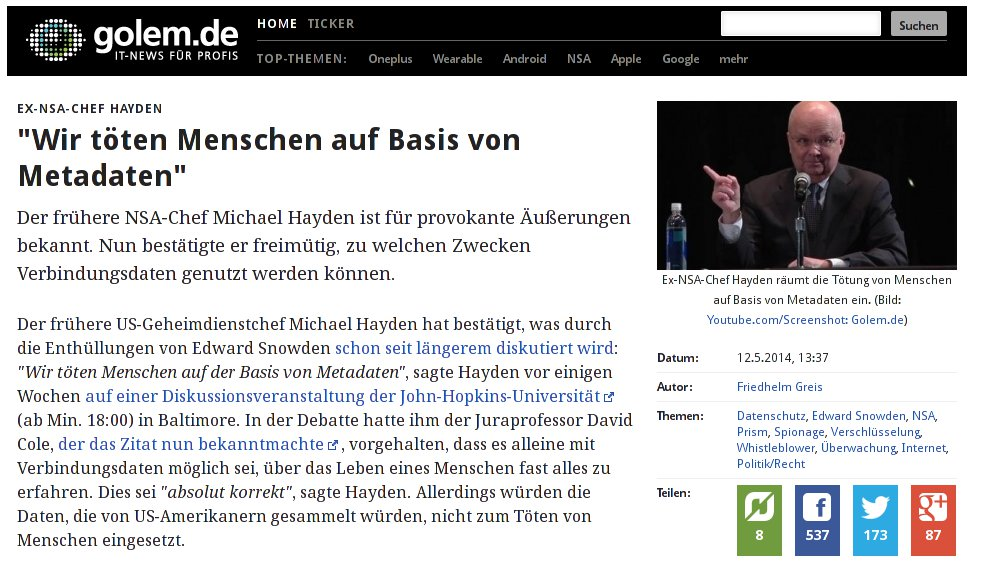
\includegraphics[height=0.7\textheight]{img/wekillpeople.jpg}
  \end{center}
\end{frame}

\begin{frame}
  \frametitle{Skynet}
  \begin{center}
    \only<2>{
      
\includegraphics[height=0.7\textheight]{img/terminator.jpg}
    }
    \only<3>{
      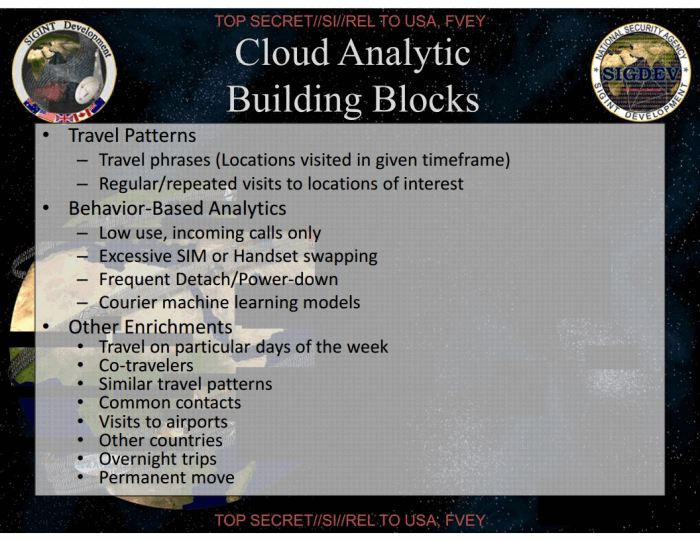
\includegraphics[height=0.7\textheight]{img/skynet.png}
    }
  \end{center}
\end{frame}

\section{Wirtschaft}
\subsection{}

\begin{frame}
  \frametitle{Google}
  \begin{center}
    
\includegraphics[height=0.4\textheight]{img/google.jpg}
  \end{center}
\end{frame}

\begin{frame}
  \frametitle{Telefonica}
  \pause
  \begin{center}
    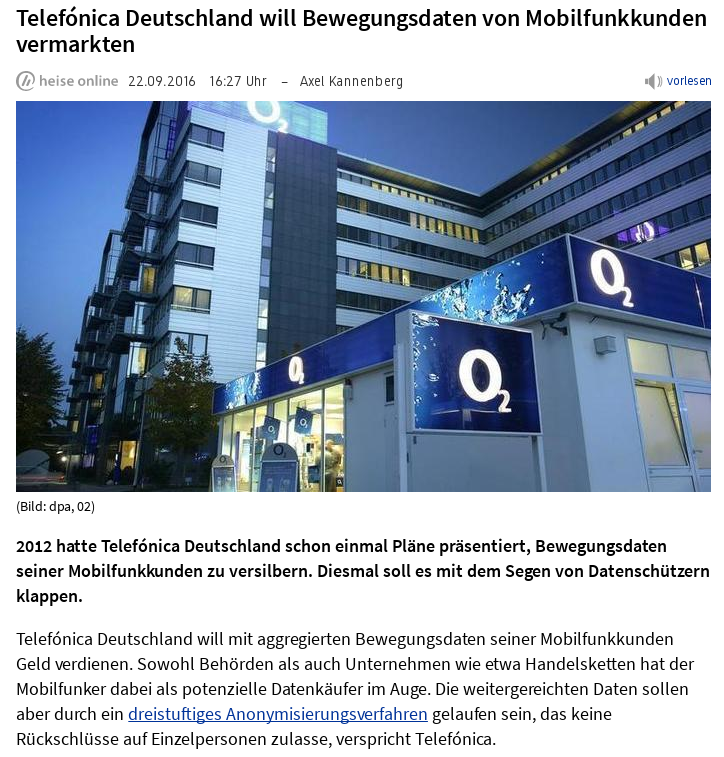
\includegraphics[height=0.7\textheight]{img/telefonica.png}
  \end{center}
\end{frame}

\begin{frame}
  \frametitle{Datenanalyse}
  \pause
  \begin{center}
    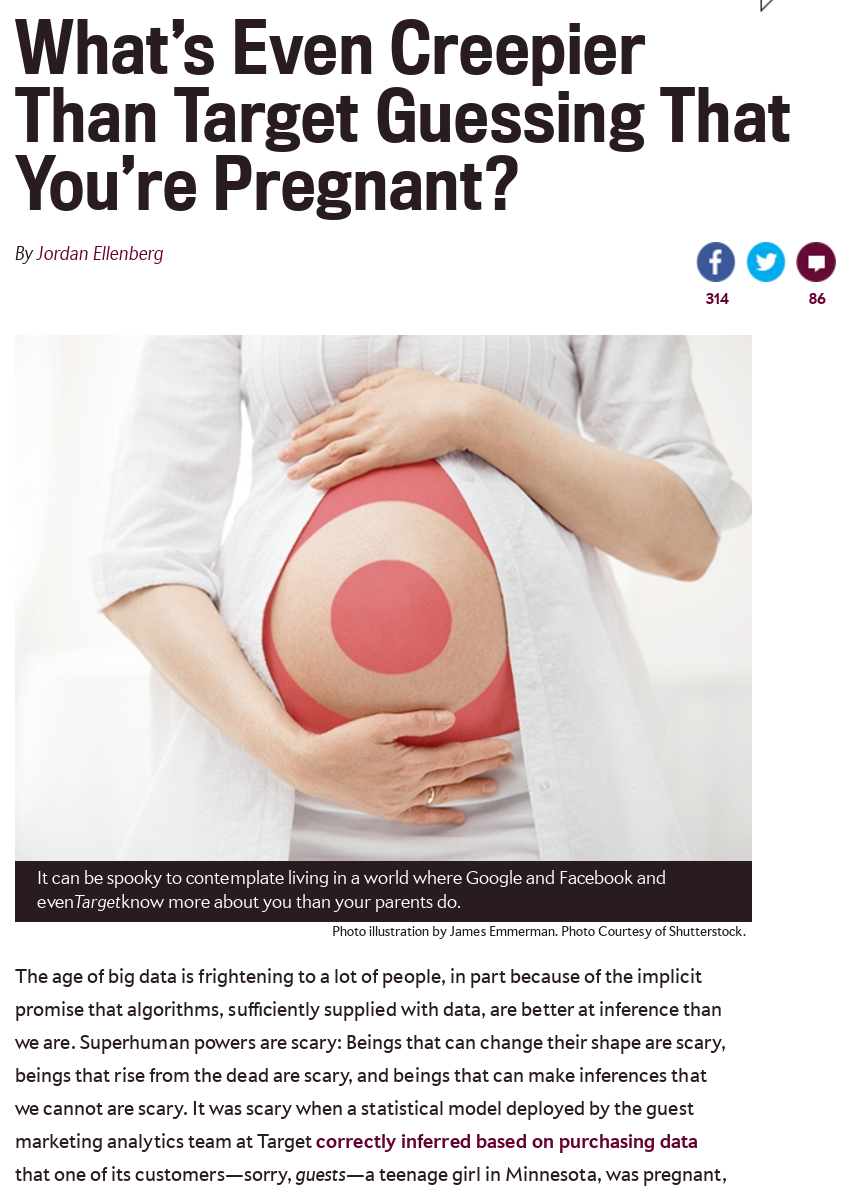
\includegraphics[height=0.8\textheight]{img/pregnant.png}
  \end{center}
\end{frame}

\begin{frame}
  \frametitle{Werbenetzwerke}
  \begin{center}
    \only<2>{
      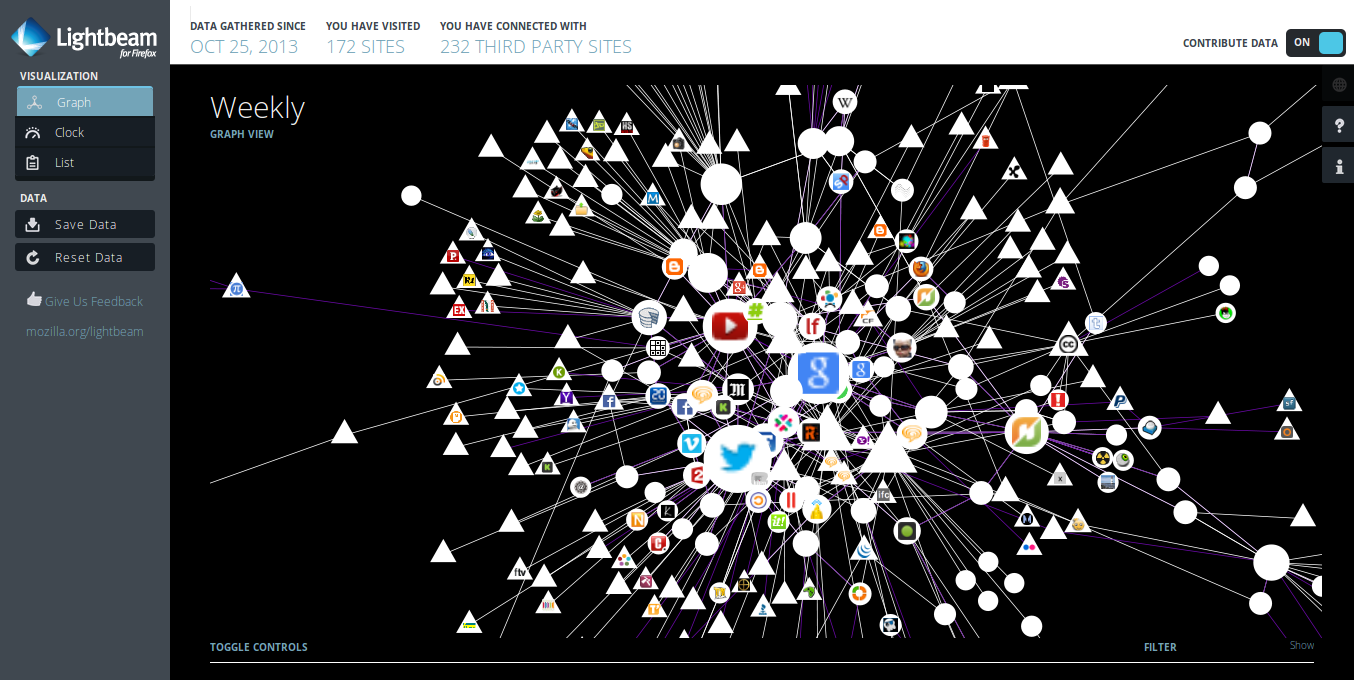
\includegraphics[height=0.7\textheight]{img/lightbeam.png}
    }
    \only<3>{
      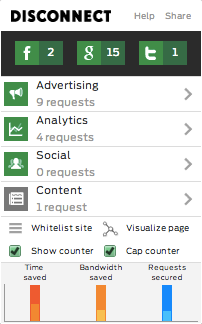
\includegraphics[height=0.7\textheight]{img/disconnect.png}
    }
  \end{center}
\end{frame}

\section{Risiken}
\subsection{}

\begin{frame}
  \frametitle{Missbrauchspotential}
  \begin{itemize}
    \item<2-> alle Daten die existieren können Missbraucht werden
    \item<3-> Angriff von Außen
    \item<4-> LOVEINT
    \item<5-> wirtschaftliche Interessen
    \item<6-> ...
  \end{itemize}
\end{frame}

\begin{frame}
  \frametitle{Verhaltensänderung}
  \begin{center}
    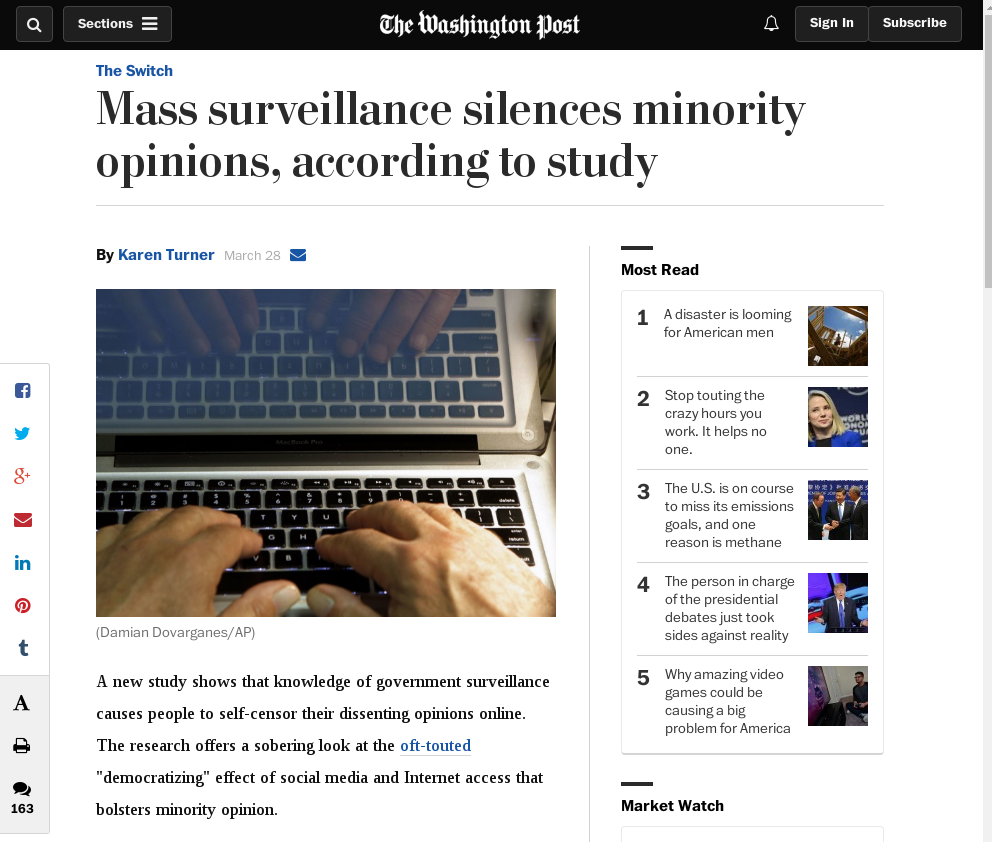
\includegraphics[height=0.7\textheight]{img/verhalten.png}
  \end{center}
\end{frame}

\section{Gegenmaßnahmen}
\subsection{}

\begin{frame}
  \frametitle{Gegenmaßnahmen}
  \pause
  \begin{center}
    \large Verschlüsselung?
  \end{center}
\end{frame}

\begin{frame}
  \frametitle{TOR}
  \begin{center}
    \only<2>{
      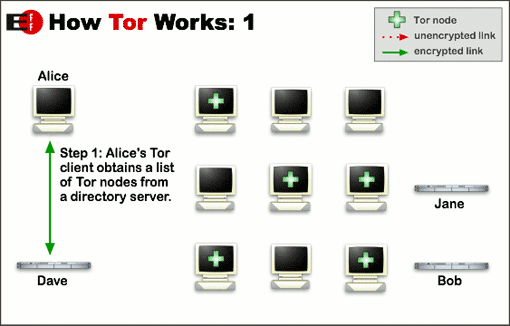
\includegraphics[height=0.7\textheight]{img/tor1.png}
    }
    \only<3>{
      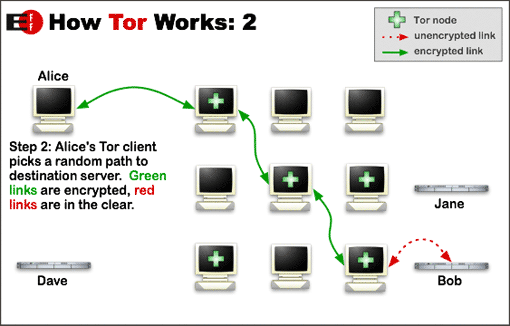
\includegraphics[height=0.7\textheight]{img/tor2.png}
    }
    \only<4>{
      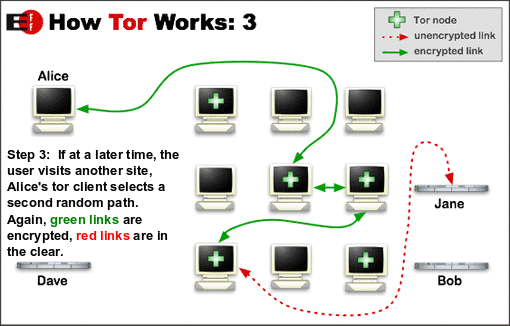
\includegraphics[height=0.7\textheight]{img/tor3.png}
    }
  \end{center}
\end{frame}

\begin{frame}
  \frametitle{Architektur von Diensten}
  \begin{itemize}
    \item<2-> zentralisierte Dienste
    \item<3-> föderalisierte Dienste
    \item<4-> peer to peer
  \end{itemize}
\end{frame}

\section{Fazit}
\subsection{}

\begin{frame}
  \frametitle{Fazit}
  \begin{itemize}
    \item<2-> schwer technisch vermeidbar
    \item<3-> immer mehr Daten
    \item<4-> hohes Missbrauchspotential
    \item<5-> Problembewusstsein
    \item<6-> Verantwortungsvoller Umgang
  \end{itemize}
\end{frame}

\end{document}
